\documentclass[11pt]{article}

\usepackage[margin=1.6cm]{geometry}
\usepackage{amsmath}
\usepackage{amssymb}
\usepackage{enumitem}
\usepackage{titlesec}
\usepackage{xcolor}
\usepackage{fancyhdr}
\usepackage{multicol}
\usepackage{array}
\usepackage{tikz}
\usetikzlibrary{arrows.meta}
\usepackage{pgfplots}
\pgfplotsset{compat=1.18}

\titleformat{\section}{\large\bfseries\color{blue!50!black}}{\thesection}{0.6em}{}
\titlespacing{\section}{0pt}{1.1em}{0.4em}
\titleformat{\subsection}{\normalsize\bfseries}{\thesubsection}{0.6em}{}
\titlespacing{\subsection}{0pt}{0.8em}{0.3em}

\setlength{\headheight}{14pt}

\pagestyle{fancy}
\fancyhf{}
\fancyhead[L]{Manipulating Functions}
\fancyfoot[C]{\thepage}
\renewcommand{\headrulewidth}{0.4pt}

\fancypagestyle{firstpage}{%
  \fancyhf{}
  \fancyhead[L]{Manipulating Functions}
  \fancyhead[R]{Name: \makebox[4cm]{\hrulefill}}
  \fancyfoot[C]{\thepage}
  \renewcommand{\headrulewidth}{0.4pt}
}

\newcommand{\ans}{\hrulefill}
\newcommand{\anshere}{\par\vspace{0.3em}\noindent\ans\par\vspace{0.3em}}
\setlist[enumerate,1]{leftmargin=1.4em, itemsep=0.4em, topsep=0.2em}
\setlength{\columnsep}{1.1cm}
\setlength{\columnseprule}{0.4pt}
\raggedcolumns

\newcommand{\gridaxis}[5]{%
  \begin{axis}[
    width=4.6cm, height=4.3cm,
    xmin=#1, xmax=#2, ymin=#3, ymax=#4,
    grid=both, grid style={line width=.1pt, draw=gray!35},
    axis lines=middle,
    xlabel={$x$}, ylabel={$y$},
    xtick distance=#5, ytick distance=#5,
    tick label style={font=\tiny},
    label style={font=\small},
    xlabel style={at={(axis description cs:1,0)}, anchor=north west},
    ylabel style={at={(axis description cs:0,1)}, anchor=south east},
    axis line style={-{Latex[length=1.8mm]}},
  ]
}

\begin{document}
\thispagestyle{firstpage}

\begin{center}
  {\Large\bfseries Manipulating Functions}\\[2pt]
  {\normalsize Extension: Building Towards Calculus}
\end{center}
\vspace{0.2em}

\section*{Fluency}

\begin{multicols}{2}
\subsection*{Substituting into $f(x)$}
\noindent Let $f(x) = x^2+3x-1$.
\vspace{0.2em}

\noindent\textbf{Worked example:} Find $f(x+2)$. Replace \emph{every} $x$ with $(x+2)$:
\begin{align*}
  f(x+2) &= (x+2)^2+3(x+2)-1 \\
         &= x^2+4x+4+3x+6-1 \\
         &= x^2+7x+9.
\end{align*}
\vspace{0.2em}
\begin{enumerate}[label=(\alph*)]
  \item $f(x-1)$
  \anshere
  \item $f(2x)$
  \anshere
  \item $f(-x)$
  \anshere
  \item $f(x+h)$
  \anshere
  \item $f(3x)$
  \anshere
  \item $f(x-4)$
  \anshere
  \item $f(-2x)$
  \anshere
\end{enumerate}

\columnbreak

\subsection*{Scaling and shifting $g(x)$}
\noindent Let $g(x) = 2x^2-x+4$.
\vspace{0.2em}

\noindent\textbf{Worked example:} Find $3g(x)$. Multiply the \emph{whole} function by $3$:
\[
  3g(x) = 3(2x^2-x+4) = 6x^2-3x+12.
\]
\vspace{0.2em}
\begin{enumerate}[label=(\alph*)]
  \item $-g(x)$
  \anshere
  \item $2g(x)+1$
  \anshere
  \item $g(x)-5$
  \anshere
  \item $-2g(x)$
  \anshere
  \item $\dfrac{1}{2}g(x)$
  \anshere
  \item $g(x)+3$
  \anshere
  \item $-g(x)-2$
  \anshere
\end{enumerate}
\end{multicols}

\newpage

\section*{Problem Solving}

\begingroup\small
\noindent Let $f(x) = 2x+1$ and $g(x) = x^2-4$ for all of Problem Solving.

\begin{multicols}{2}
\subsection*{Composite functions with numbers}
\noindent\textbf{Worked example:} Find $f(g(2))$. Work from the \emph{inside out}: first find
$g(2)$, then substitute that result into $f$.
\[
  g(2) = 2^2-4 = 0, \qquad f(g(2)) = f(0) = 2(0)+1 = 1.
\]
\vspace{0.2em}
\begin{enumerate}[label=(\alph*)]
  \item $g(f(2))$
  \anshere
  \item $f(g(-3))$
  \anshere
  \item $g(f(0))$
  \anshere
\end{enumerate}

\columnbreak

\subsection*{Composite functions with algebra}
\noindent\textbf{Worked example:} Find $f(g(a))$. Substitute the \emph{whole} expression for
$g(a)$ into $f$, then expand and simplify:
\[
  f(g(a)) = f(a^2-4) = 2(a^2-4)+1 = 2a^2-8+1=2a^2-7.
\]
\vspace{0.2em}
\begin{enumerate}[label=(\alph*)]
  \item $g(f(a))$
  \anshere
\end{enumerate}

\vspace{0.6em}
\subsection*{Interpreting scenarios}
\begin{enumerate}[label=(\alph*)]
  \item A clothing shop sells shirts for \$25 each. The function $C(n)=25n$ gives the cost (\$)
    of buying $n$ shirts before tax. The function $T(c)=1.15c$ adds 15\% GST to a cost $c$.
    Calculate $T(C(4))$, and explain in words what this number represents.
  \anshere
  \item A car travels at $80$\,km/h. The function $d(t)=80t$ gives the distance (km) travelled
    after $t$ hours. The function $p(d)=0.12d$ gives the fuel cost (\$) for travelling a distance
    $d$\,km. Calculate $p(d(2.5))$, and explain in words what this number represents.
  \anshere
\end{enumerate}
\end{multicols}
\endgroup

\newpage

\section*{Reasoning}

\subsection*{Composite functions are not commutative}
\noindent In general, $f(g(x)) \ne g(f(x))$ --- the order you apply two functions matters.

\vspace{0.3em}
\noindent\textbf{Worked example:} Using $f(x)=3x^2+2$ and $g(x)=5x$, show that
$f(g(x)) \ne g(f(x))$.
\begin{align*}
  f(g(x)) &= f(5x) = 3(5x)^2+2 = 3(25x^2)+2 = 75x^2+2. \\
  g(f(x)) &= g(3x^2+2) = 5(3x^2+2) = 15x^2+10.
\end{align*}
Since $75x^2+2 \ne 15x^2+10$ for all $x$, we have shown $f(g(x)) \ne g(f(x))$.

\vspace{0.4em}
\begin{enumerate}[label=(\alph*)]
  \item Using $f(x) = x^2-1$ and $g(x) = x+3$, show that $f(g(x)) \ne g(f(x))$.
  \anshere
  \item Using $f(x) = x+4$ and $g(x) = x^2$, show that $f(g(x)) \ne g(f(x))$.
  \anshere
\end{enumerate}

\vspace{0.6em}
\subsection*{Finding the inverse function $f^{-1}(x)$}
\noindent The inverse function $f^{-1}(x)$ ``undoes'' $f(x)$. To find it: write $y=f(x)$, swap
$x$ and $y$, then solve for $y$.

\vspace{0.3em}
\noindent\textbf{Worked example:} Find $f^{-1}(x)$ for $f(x) = 2x+5$.
\begin{align*}
  y &= 2x+5 & &\text{(write as $y=\ldots$)}\\
  x &= 2y+5 & &\text{(swap $x$ and $y$)}\\
  x-5 &= 2y \\
  y &= \frac{x-5}{2} & &\text{(solve for $y$)}
\end{align*}
So $f^{-1}(x) = \dfrac{x-5}{2}$.

\vspace{0.4em}
\begin{multicols}{2}
\begin{enumerate}[label=(\alph*)]
  \item $f(x) = 4x-3$
  \anshere
  \item $f(x) = -2x+7$
  \anshere
  \item $f(x) = \dfrac{x+6}{3}$
  \anshere
  \item $f(x) = \dfrac{2x-5}{4}$
  \anshere
  \item[(e)] \textbf{Bonus:} $f(x) = x^3+1$
  \anshere
\end{enumerate}
\end{multicols}

\newpage

\section*{Enrichment}

\begingroup\small
\subsection*{The difference quotient --- towards the derivative}
\noindent In calculus, the expression $\dfrac{f(x+h)-f(x)}{h}$ measures the \emph{average rate of
change} of $f$ between $x$ and $x+h$. As $h$ gets closer and closer to $0$, this expression
approaches the \textbf{derivative} of $f$ at $x$, written $f'(x) = \displaystyle\lim_{h\to 0}
\frac{f(x+h)-f(x)}{h}$.

\vspace{0.3em}
\noindent\textbf{Worked example:} Find $\dfrac{f(x+h)-f(x)}{h}$ for $f(x)=x^2$, then state what
it approaches as $h\to 0$.
\begin{align*}
  f(x+h)-f(x) &= (x+h)^2-x^2 = x^2+2xh+h^2-x^2 = 2xh+h^2. \\
  \frac{f(x+h)-f(x)}{h} &= \frac{2xh+h^2}{h} = 2x+h.
\end{align*}
As $h\to 0$, $2x+h \to 2x$. So $f'(x) = 2x$.

\vspace{0.4em}
\begin{multicols}{2}
\noindent For each $f(x)$: find and simplify $\dfrac{f(x+h)-f(x)}{h}$, then state what it
approaches as $h\to 0$.
\begin{enumerate}[label=(\alph*)]
  \item $f(x) = x^2+3x$
  \anshere
  \item $f(x) = 2x^2-5$
  \anshere
  \item $f(x) = x^3$
  \anshere
  \item $f(x) = 4x+7$
  \anshere
\end{enumerate}
\end{multicols}

\vspace{0.4em}
\subsection*{Transforming graphs: $f(x-h)-v$}
\noindent Replacing $x$ with $(x-h)$ shifts the graph of $f$ \textbf{$h$ units right}.
Subtracting $v$ shifts the graph \textbf{$v$ units down}. (A negative $h$ or $v$ shifts the
\emph{other} way.)

\vspace{0.3em}
\noindent\textbf{Worked example:} For $f(x)=x^2$ with $h=3$ and $v=2$:
\[
  f(x-h)-v = (x-3)^2-2.
\]
Graph $y=f(x)$ and $y=(x-3)^2-2$ in Desmos (or sketch them on the same grid below). You should
see the second graph is the first one shifted $3$ units right and $2$ units down.

\begin{center}
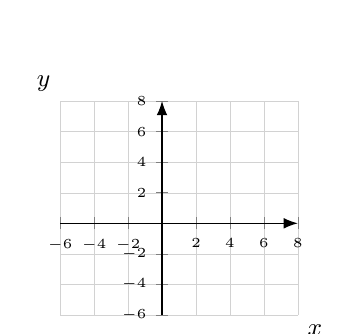
\begin{tikzpicture}
\gridaxis{-6}{8}{-6}{8}{2}
\end{axis}
\end{tikzpicture}
\end{center}

\vspace{0.4em}
\noindent For each function below: (i) write the expression for $f(x-h)-v$, (ii) graph $y=f(x)$
and $y=f(x-h)-v$ in Desmos, and (iii) describe the transformation you see.

\begin{enumerate}[label=(\alph*)]
  \item $f(x) = x^3$, with $h=2$, $v=1$.
  \anshere
  \item $f(x) = |x|$, with $h=4$, $v=-3$.
  \anshere
  \item $f(x) = \sqrt{x}$, with $h=1$, $v=4$.
  \anshere
\end{enumerate}
\endgroup

\end{document}
